\section{Classification}

\begin{mdframed}
    \textbf{Linear Classification:} used to determine to which discrete category a specific example belongs. (classification of emails into spam or ham)
\end{mdframed}
Output category:
\begin{itemize}
    \item \textbf{Binary classification:} 2 possible categories
    \item \textbf{Multi-class classification:} n possible categories
\end{itemize}
We can use binary classification by applying a threshold:
\begin{itemize}
    \item $h_\theta(x) = \theta^Tx$
    \item if $h_\theta(x) \geq 0$, then the output is $y = 1$
    \item if $h_\theta(x) < 0$, then the output is $y = -1$
\end{itemize}
\begin{equation} \tag{Classification}
    y = sign(h_\theta(x))
\end{equation}
Applying Linear Regression, for classification task, is not a good idea. Instead, it is preferable to use Logistic Regression, which, despite containing regression in its name, is a classification algorithm.
\begin{center}
    \begin{tabular}{c}
        \\ 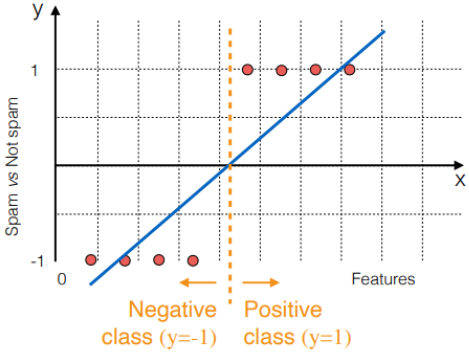
\includegraphics[width=0.5\textwidth]{images/Classification1.png} \\ \\
    \end{tabular}
\end{center}
For larger dimensions, we assume a straight line, a shift of a certain term (bias term):
\begin{center}
    \begin{tabular}{c}
        \\ 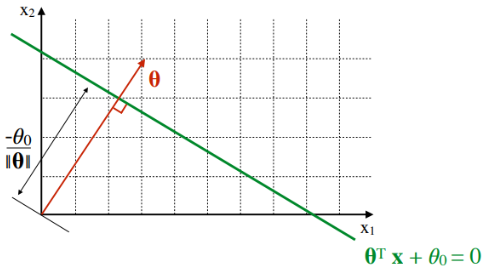
\includegraphics[width=0.5\textwidth]{images/Classification2.png} \\ \\
    \end{tabular}
\end{center}
We then estimate a good decision boundary by deciding the direction $\theta$ and position $\theta_0$ of the boundary, and we need a parameter selection criterion. For example, the Loss Functions.

\subsection{Loss Functions}
\begin{equation} \tag{Zero/One}
    J_{01}(\theta) = \cfrac{1}{m} \sum_{i=1}^m \{ 0 \text{ if } h_\theta(x_i) = y_i, \text{else } 1 \}
\end{equation}
\begin{equation} \tag{Absolute}
    J_{abs}(\theta) = \cfrac{1}{m} \sum_{i=1}^m | h_\theta(x_i) - y_i |
\end{equation}
\begin{equation} \tag{Squared}
    J_{sqr}(\theta) = \cfrac{1}{2m} \sum_{i=1}^m (h_\theta(x_i) - y_i )^2
\end{equation}
The loss function for the Logistic Regression is:
\begin{equation} \tag{Loss function}
    J(\theta) = \cfrac{1}{m} \sum_{i=1}^m \text{cost}(h_\theta(x_i, y_i))
\end{equation}
where:
\begin{equation} \tag*{}
    \text{cost}(h_\theta(x_i, y_i)) =
    \begin{cases}
        -\log(h_\theta(x_i)) \quad \text{if } y_i = 1 \\
        -\log(1 - h_\theta(x_i)) \quad \text{if } y_i = 0
    \end{cases}
\end{equation}
Because this function is convex, we can use gradient descent. In fact, the method used to calculate the Linear Regression loss would not be correct in a convex function if used with the Logistic Regression function.

\newpage